% DSAI4102 final report. Compile on Overleaf (IEEEtran is built in): upload this folder, then Recompile.
% Every number comes from outputs/events/key_numbers_events.json (events.ipynb) or
% outputs/final/key_numbers.json (final_project.ipynb). Figures are refreshed by make_slide_figures.py.
\documentclass[conference]{IEEEtran}
\IEEEoverridecommandlockouts
\usepackage{cite}
\usepackage{amsmath,amssymb}
\usepackage{graphicx}
\usepackage{booktabs}
\usepackage{url}
\usepackage[hidelinks]{hyperref}
\graphicspath{{figures/}}
\renewcommand{\topfraction}{0.9}
\renewcommand{\dbltopfraction}{0.9}
\renewcommand{\floatpagefraction}{0.8}
\renewcommand{\dblfloatpagefraction}{0.8}
\setlength{\emergencystretch}{1.5em}

\begin{document}

\title{Which Events Change How Stocks Move Together,\\ and Do the Changes Last?\\ Event-Matched Association Rule Mining on 40 US Stocks, 2016--2026}

\author{
\IEEEauthorblockN{Farid Abdul Rehman (60304642), Muzayyan Parkar (60305825), Mohamad Zain (60306080)}
\IEEEauthorblockA{DSAI4102 Applied Data Mining, Department of Data Science and AI\\
University of Doha for Science and Technology, Doha, Qatar\\
Instructor: Moshiur Rahman Farazi}
}

\maketitle

\begin{abstract}
Stocks move together in habits, and a portfolio is riskier than it looks if news quietly rewires those habits. We mine co-movement rules for 40 US stocks (AI chip makers, Big Tech, traditional software and a non-tech control group) from 2,733 daily baskets of market-adjusted major moves, 2016 to November 2026, and ask which of 368 dated events (Federal Reserve decisions, CPI and jobs reports, 19 one-off shocks) and 1,744 earnings reactions line up with unusual days and structure breaks, and whether the breaks last. Unusual days and breaks are found without labels, by an Isolation Forest and a weekly break score, and are then matched to events against 1,000 shifted calendars. Removing the market first matters most: raw-return rules mostly restate market volatility (median 3,905 rules per window against 118). Scheduled releases explain unusual days no better than chance (11\% against 13\%); the match rate reaches 41\% (chance 14\%, $p=0.001$) only through hand-picked shocks. Fed days stand out for one stock, the bank JPM (1.52 times its usual rate of major moves). Shocks do not land on structure breaks ($p=0.26$), and of 15 shocks that can be followed for two years, 12 leave no break, 3 leave a lasting one and none leaves a break that heals. The lasting change we do find, which stocks the market treats as AI stocks, built up over three years without a single break date.
\end{abstract}

\begin{IEEEkeywords}
association rules, FP-Growth, event analysis, anomaly detection, change mining, stock co-movement
\end{IEEEkeywords}

\section{Introduction}
Investors diversify by holding stocks that do not move together. If an event makes two ``unrelated'' stocks start moving together, a portfolio carries more risk than its holder believes. The useful questions are therefore which events rewire who moves with whom, whether a manager should react to every big news day, and which co-movement patterns can be relied on. Association rule mining~\cite{agrawal1993} suits these questions because it finds combinations of stocks that make large moves on the same day, including combinations of three, not only pairwise correlations.

Our proposal asked whether one event, ChatGPT's release, changed co-movement. The feedback asked how we would know a change came from that event and not from the market or from everything else that happened at the same time. We therefore stopped assuming that one date matters and test every dated event the same way, against chance. The data mining rationale is \emph{pattern discovery}: rules, unusual days and structure breaks are found without labels, and only then compared with an event calendar. Prediction is used in service of the patterns: its target is whether a mined rule lasts.

Before running the event tests we wrote down six hypotheses, each with a result that could prove it wrong (Table~\ref{tab:scorecard}): H1, unusual days and breaks fall on events more often than chance; H1a, a company's earnings move its own group; H1b, rate and inflation news moves rate-sensitive stocks rather than tech; H1c, at least half of the top 1\% unusual days match an event; H1d, AI product launches do not break the structure while AI business news does; H2, most breaks are temporary. H1d was written after the AI events had been scored in an earlier analysis, so it confirms that result rather than testing it afresh.

Our contributions are:
\begin{enumerate}
\item A rolling-window rule-mining baseline on market-model residual moves, with evidence that raw-return rules mostly track market volatility.
\item Label-free detection of unusual days and structure breaks, matched to 368 dated events and to earnings with an event-date shift test that keeps the calendar's rhythm.
\item A recovery-curve test of whether breaks last, measured against the normal drift of the structure.
\item Two supporting results: the market's ``AI category'' was redrawn gradually, and a rule's history and scope, not its lift, predict whether it lasts.
\end{enumerate}

\section{Related Work}
\textbf{Association rules on markets.} Kartal et al.~\cite{kartal2022} apply Apriori to up/down days of 11 world indices as one pooled dataset; Dai et al.~\cite{dai2024} compare Apriori, FP-Growth and Eclat on rises and falls of foreign indices and Taiwanese stocks with next-day lags; Chen et al.~\cite{chen2022} mine weighted inter-transaction rules to predict direction. All three treat the rule set as fixed over the sample and use raw up/down labels, so a market-wide day counts as co-movement, and none asks what changes the rules. We remove the market first, mine many windows to study change, and tie changes to dated events.

\textbf{Events and stock prices.} Event studies~\cite{mackinlay1997} measure a firm's abnormal return around a date. For scheduled macroeconomic news, Bernanke and Kuttner~\cite{bernanke2005} find that a surprise 25-basis-point rate cut lifts broad indexes by about 1\%, Savor and Wilson~\cite{savor2013} find higher average market returns on days with scheduled inflation, unemployment or rate news, and Lucca and Moench~\cite{lucca2015} find that US equities earn large excess returns ahead of Fed decisions while other macroeconomic releases show no such effect. Brenner et al.~\cite{brenner2009} study the volatility and co-movement of US financial markets around macroeconomic announcements, and Foster~\cite{foster1981} shows that one firm's earnings release moves other firms in its industry. These studies measure average returns of an index or a firm on known dates. We ask a different question, whether events change the joint structure of who moves with whom, and we let unsupervised detectors pick the dates before any calendar is consulted.

\textbf{Co-movement structure and its change.} Mantegna~\cite{mantegna1999} builds a hierarchical tree of stocks from correlations and Onnela et al.~\cite{onnela2003} track how it reorganises over time. Forbes and Rigobon~\cite{forbes2002} warn that correlations rise mechanically with volatility; our raw-versus-residual comparison is a data mining version of that warning. Barberis et al.~\cite{barberis2005} show \emph{category-based} co-movement: stocks added to an index start moving with it. Emerging patterns~\cite{dong1999} and change mining~\cite{bottcher2008} treat the evolution of patterns as the object of study, and Webb~\cite{webb2007} recommends correcting rule significance for the whole search space, which we do with Benjamini--Hochberg control~\cite{benjamini1995}. Unusual days are scored with an Isolation Forest~\cite{liu2008}.

\section{Methodology}
\begin{figure*}[!t]
\centering
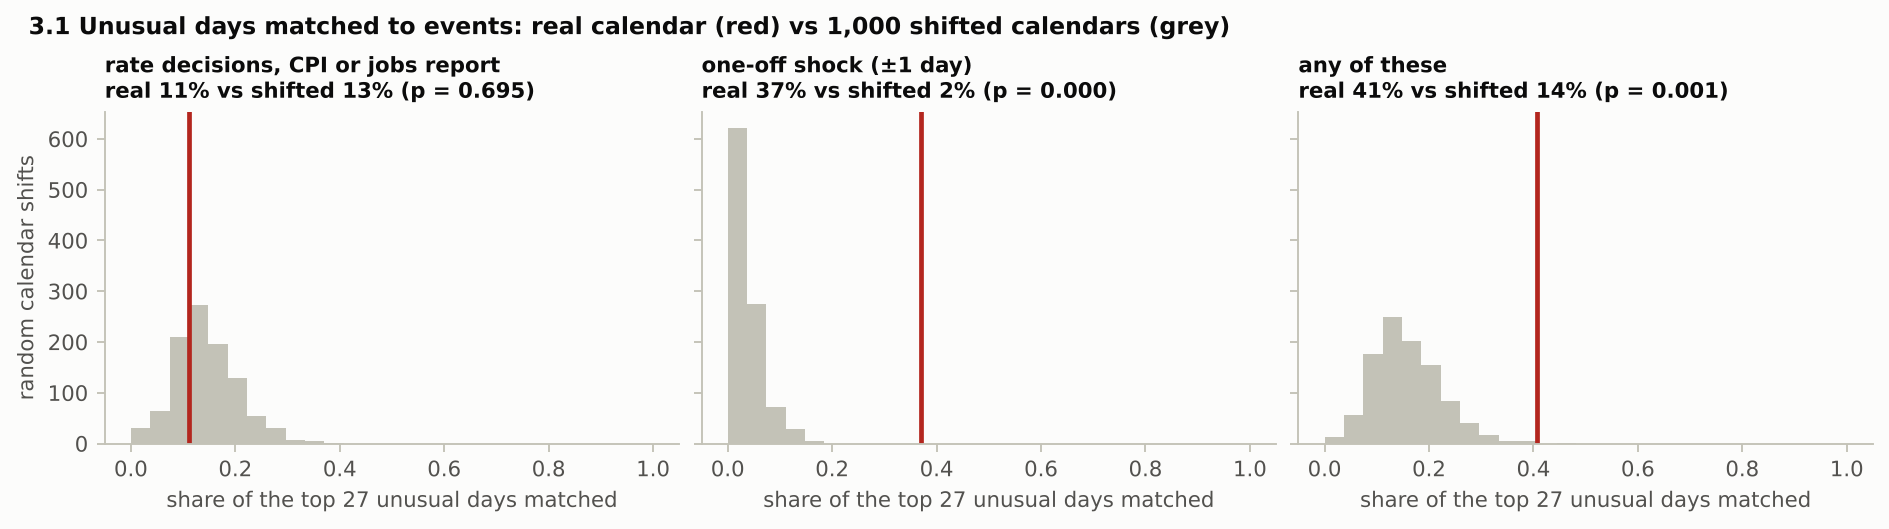
\includegraphics[width=0.86\textwidth]{3_1_unusual_days_shift_test.png}\\[2pt]
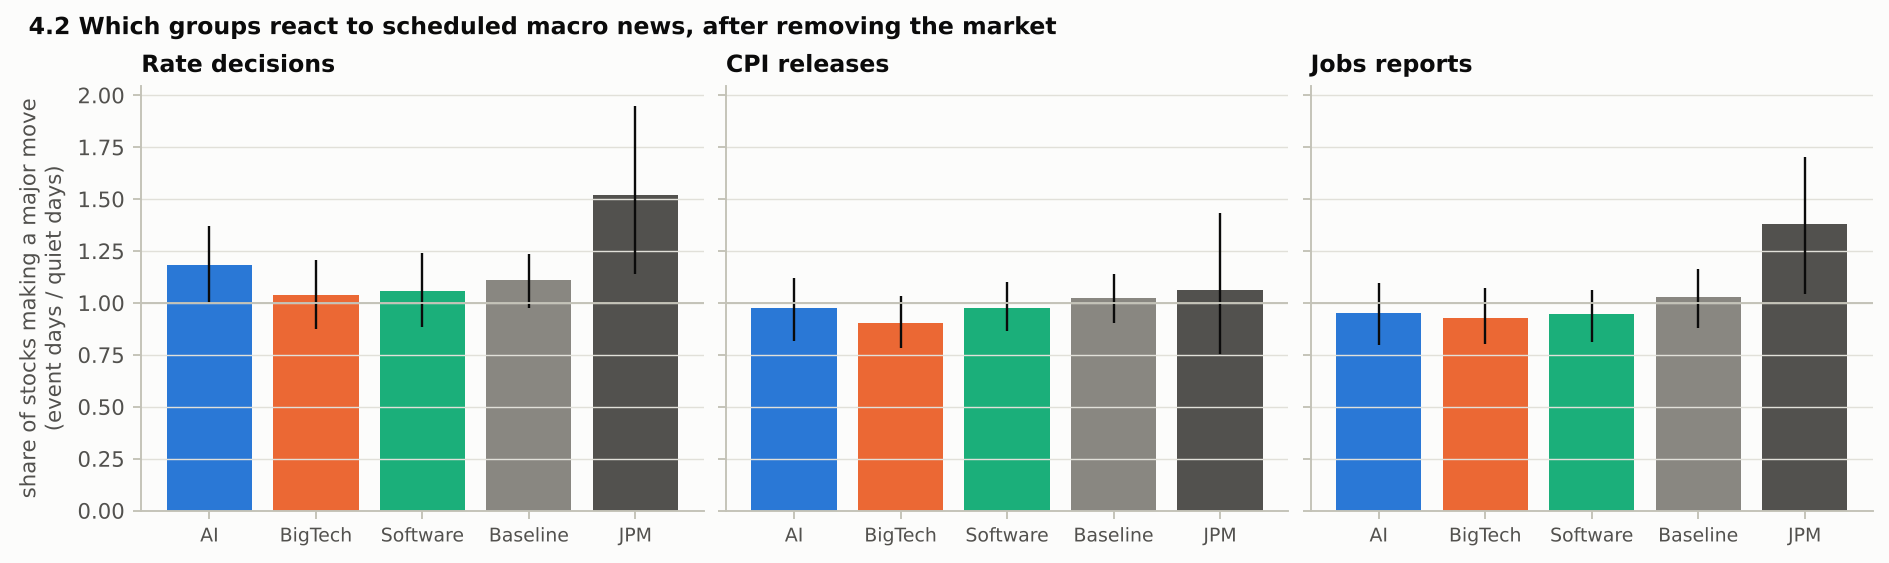
\includegraphics[width=0.86\textwidth]{4_2_move_ratio_by_group.png}
\caption{Top: share of the 27 unusual days that match each type of event, real calendar (red line) against 1,000 shifted calendars (grey). Bottom: share of each group's stocks making a major move on event days divided by the share on quiet days (1 = no difference), with 95\% bootstrap intervals.}
\label{fig:shift}
\end{figure*}

Two notebooks run top to bottom~\cite{repo}: \texttt{final\_project.ipynb} builds the items, baseline rules, anomaly scores and supporting analyses (about 5 minutes), and \texttt{events.ipynb} runs every event test (about 30 seconds).

\subsection{Data}
Daily adjusted closes for 40 stocks and the SPY ETF come from Yahoo Finance via \texttt{yfinance}~\cite{yfinance}, 2 June 2014 to 13 November 2026 (3,134 days, no missing values). The stocks form four groups: AI enablers (NVDA, AMD, AVGO, TSM, MU, QCOM, INTC, AMAT, LRCX, ASML), Big Tech (AAPL, MSFT, GOOGL, AMZN, META, ORCL, NFLX, TSLA), traditional software (ADBE, CRM, IBM, CSCO, CHGG, INTU, SAP, ACN, NOW, WDAY, ADSK, CTSH) and a non-tech control group (JPM, XOM, JNJ, PG, KO, WMT, UNH, CAT, HD, PFE). Data from 2014--2015 only estimates betas and volatilities; baskets start on 4 January 2016 (2,733 baskets).

The event calendar (\texttt{build\_events.py}) holds 88 FOMC rate decisions from the Federal Reserve's calendars, including the two emergency cuts of March 2020; 130 CPI releases and 130 jobs reports from the Bureau of Labor Statistics archives, including the delays of the 2025 government shutdown; and 19 one-off shocks (elections, the COVID crash, the 2018 and 2025 tariffs, five AI events and others), each linked to a news report or official release confirming the date. Scheduled dates are fixed in advance, so nobody chose them because the market moved; the shocks were chosen by hand after the fact and are always reported separately. Earnings dates for all 40 stocks (1,744 reaction days) come from Yahoo Finance. Every event is placed on the first trading day the market could react: a Sunday announcement counts on Monday, and an earnings report at or after the 4 p.m.\ close counts the next day.

\subsection{Items and baseline rules}
For stock $i$ on day $t$ the residual return is $e_{i,t} = r_{i,t} - \beta_{i,t}\, r_{m,t}$, with $r_m$ SPY's return and $\beta_{i,t}$ estimated over days $t-252$ to $t-1$, the market model of event studies~\cite{mackinlay1997}. Raw returns and simple excess returns are run for comparison. With $\sigma_{i,t}$ the standard deviation of $e_i$ over the previous 60 days, day $t$'s basket contains \texttt{NVDA\_UP} if $e_{i,t}/\sigma_{i,t} \geq 1$ and \texttt{NVDA\_DOWN} if it is $\leq -1$. Both $\beta$ and $\sigma$ use only earlier days, so there is no look-ahead. Baskets hold 9.6 of 80 possible items on average.

Rules are mined with FP-Growth~\cite{han2000} (\texttt{mlxtend}~\cite{raschka2018}) on 120 rolling windows of 252 baskets moved forward 21 days at a time, with minimum support 0.04 (about 10 days per window), confidence 0.4, lift 1.5 and at most three items. Two checks ask whether the rules are real: a shuffle test that permutes each item column independently (supports stay, links between stocks are destroyed), and a one-sided Fisher exact test per rule with Benjamini--Hochberg control at 5\% over all 480,480 rules of two or three items the miner could have returned~\cite{webb2007}. Pair lift, used throughout, is the lift of ``both stocks made a major move in the same direction on the same day''; 40 stocks give 780 pairs.

\subsection{Unusual days and the event-date shift test}
An Isolation Forest~\cite{liu2008} (300 trees) scores every day from its 40 residual $z$-scores (clipped at $\pm10$); the top 1\% are 27 unusual days. A day matches a scheduled release on the same day or a shock within $\pm1$ trading day, because news often breaks the evening before. Chance is measured by the \emph{event-date shift test}: the whole calendar is moved forward by a random number of trading days (at least 21, wrapping around at the end) and the matches are counted again, 1,000 times. Moving the whole calendar keeps its rhythm (eight Fed meetings a year, monthly releases) and breaks only its link to market days; random dates would not. Each unusual day also receives one descriptive category, the first rule that applies: shock, scheduled release, earnings reaction (a company reporting that day is among the five largest residual moves), market stress (SPY's trailing 21-day volatility in its top 5\%), earnings day with a quiet reporter, or unexplained.

\subsection{Who reacts to scheduled news}
Each event type's anomaly scores are compared with \emph{quiet days} (no release and no shock within a day) by a one-sided Mann--Whitney test, with Benjamini--Hochberg across the four types. For each group, the share of its stocks making a major move on event days is divided by the same share on quiet days; 1.0 means no difference, and since the market is already removed, a ratio above 1 means a reaction beyond the stock's usual market sensitivity. Intervals are 95\% bootstrap intervals over event days (500 resamples). Events also enter the rules as items: for a left-hand side such as \texttt{FOMC\_DAY}, rules are mined from the conditional database of that event's baskets (consequent on at least 25\% and at least five of those days, lift $\geq1.5$), tested with Fisher's test, and corrected over every single and pair right-hand side that could have been tested. For earnings, the left-hand side is ``company $T$ reported and made a major move'', e.g.\ \{\texttt{EARN\_NVDA}, \texttt{NVDA\_UP}\}, and each rule's lift is compared with the lift after the same company's major moves on days without its earnings, so a rule counts only if earnings add something to ordinary co-movement.

\subsection{Structure breaks and recovery curves}
The \emph{local break score} at a date is $1-\rho$, where $\rho$ is the correlation between the 780 $\log_2$ pair lifts of the half-year (126 baskets) before the date and the half-year after it, computed weekly. Break peaks are local maxima above the 90th percentile at least a quarter apart. Whether shocks land on breaks is tested by the shocks' mean percentile against 1,000 shifted shock calendars.

For H2, the half-year before each shock is its ``normal'' structure, and we measure the similarity (correlation of pair lifts) between it and half-years starting 0, 21, \dots, 504 trading days after the shock. Similarity falls with distance even without any event, so the same calculation is started at every month of the sample to give the \emph{normal drift}, and each value is expressed in standard deviations from it. The rule, fixed before running, is: \emph{no break} if the lowest value in the first quarter is above $-1$; \emph{temporary} if it dips below $-1$ and the second-year mean returns above $-0.5$; \emph{lasting} if the second-year mean stays at $-1$ or below; \emph{too recent} if fewer than four second-year points exist. The test is run on all pairs and on pairs that include an AI enabler.

\subsection{Supporting analyses}
A stock's \emph{AI affinity} is its mean pair lift with the ten AI enablers; its change between the two years before ChatGPT and the latest two years gets a 95\% moving-block bootstrap interval~\cite{kunsch1989} (10-day blocks, 500 resamples) and Benjamini--Hochberg control across stocks. For rule survival, a rule mined from the window ending on day $t$ \emph{survives} if it passes the same thresholds in the next 126 baskets, which do not overlap its window. Twenty features known on day $t$ (strength measures, number of groups spanned, age in consecutive earlier windows, burstiness, market volatility) feed logistic regression, a random forest and gradient boosting (scikit-learn~\cite{pedregosa2011}), trained on 8,202 rules whose future ends before 30 November 2022 and tested on 5,215 later ones, against one-feature baselines.

\subsection{Robustness settings}
The event tests are repeated with a stricter major move ($z\geq1.5$) and with raw returns.

\section{Results and Discussion}
\begin{figure*}[!t]
\centering
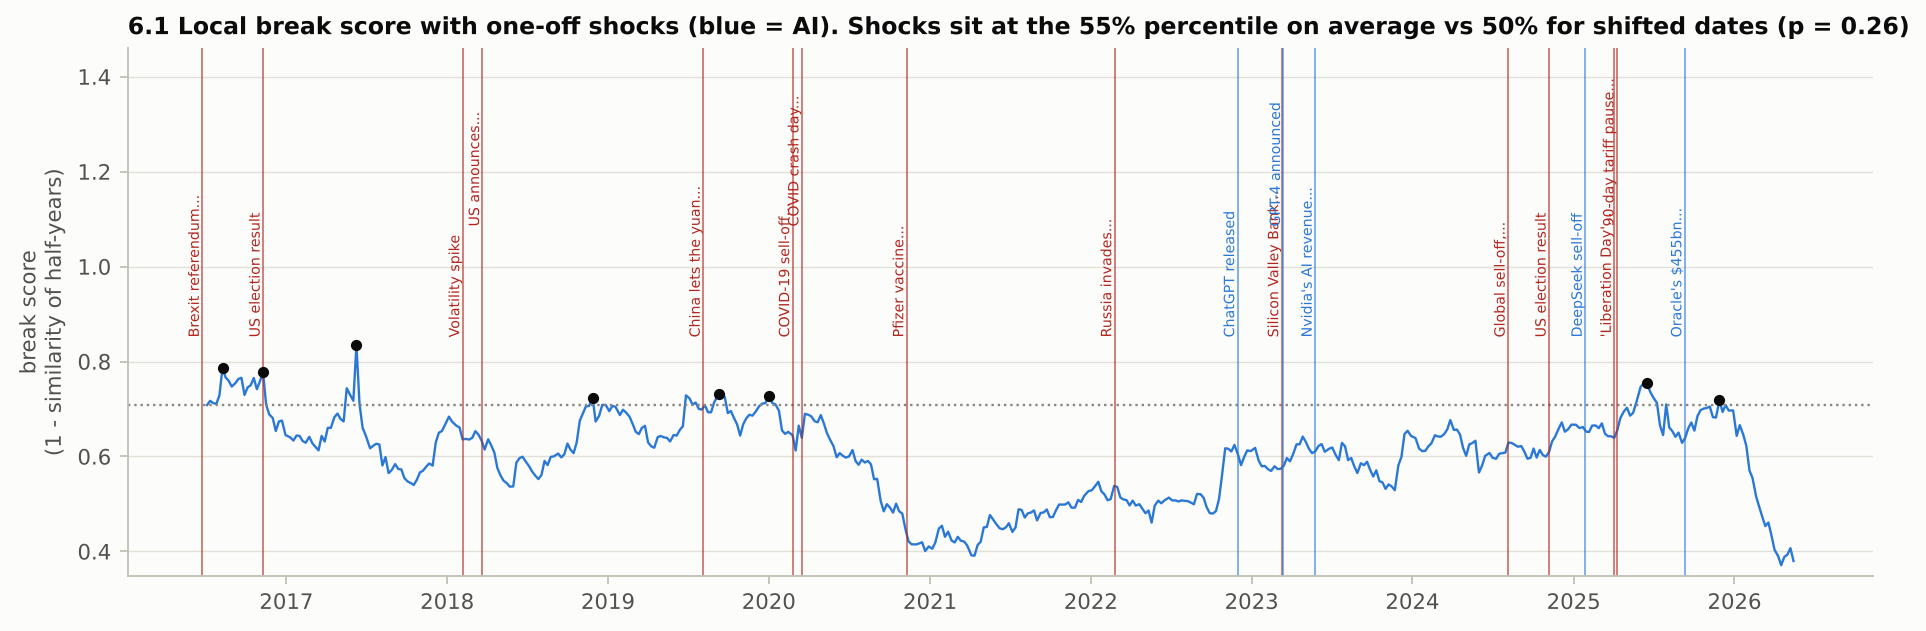
\includegraphics[width=0.9\textwidth]{6_1_local_breaks_and_shocks.png}
\caption{Weekly local break score (1 $-$ correlation of the 780 pair lifts in the half-year before and after) with one-off shocks; blue lines are AI events. Dots mark break peaks; the dotted line is the 90th percentile.}
\label{fig:breaks}
\end{figure*}


\subsection{Removing the market changes what is found}
Under raw returns the rule count reaches 51,138 in one 2020 window and follows market volatility (Spearman 0.71 between a window's rule count and SPY volatility; median 3,905 rules). Under residual returns the median is 118 and the correlation 0.37 (Fig.~\ref{fig:rules}). About 97\% of raw rules therefore restate that the market moved. Shuffled baskets produce 67 rules against 24,585 real ones (0.3\%), and 82\% of real rules survive the Fisher test corrected for all possible rules, so the residual rules are not search artefacts. Without this step every crash would look like a structure break and every crash day like an event effect. FP-Growth and Apriori returned identical itemsets. At our limit of three items Apriori was several times faster; FP-Growth was three to four times faster only when five-item rules were allowed on the raw 2020 window, where Apriori's candidates explode.

\begin{figure}[t]
\centering
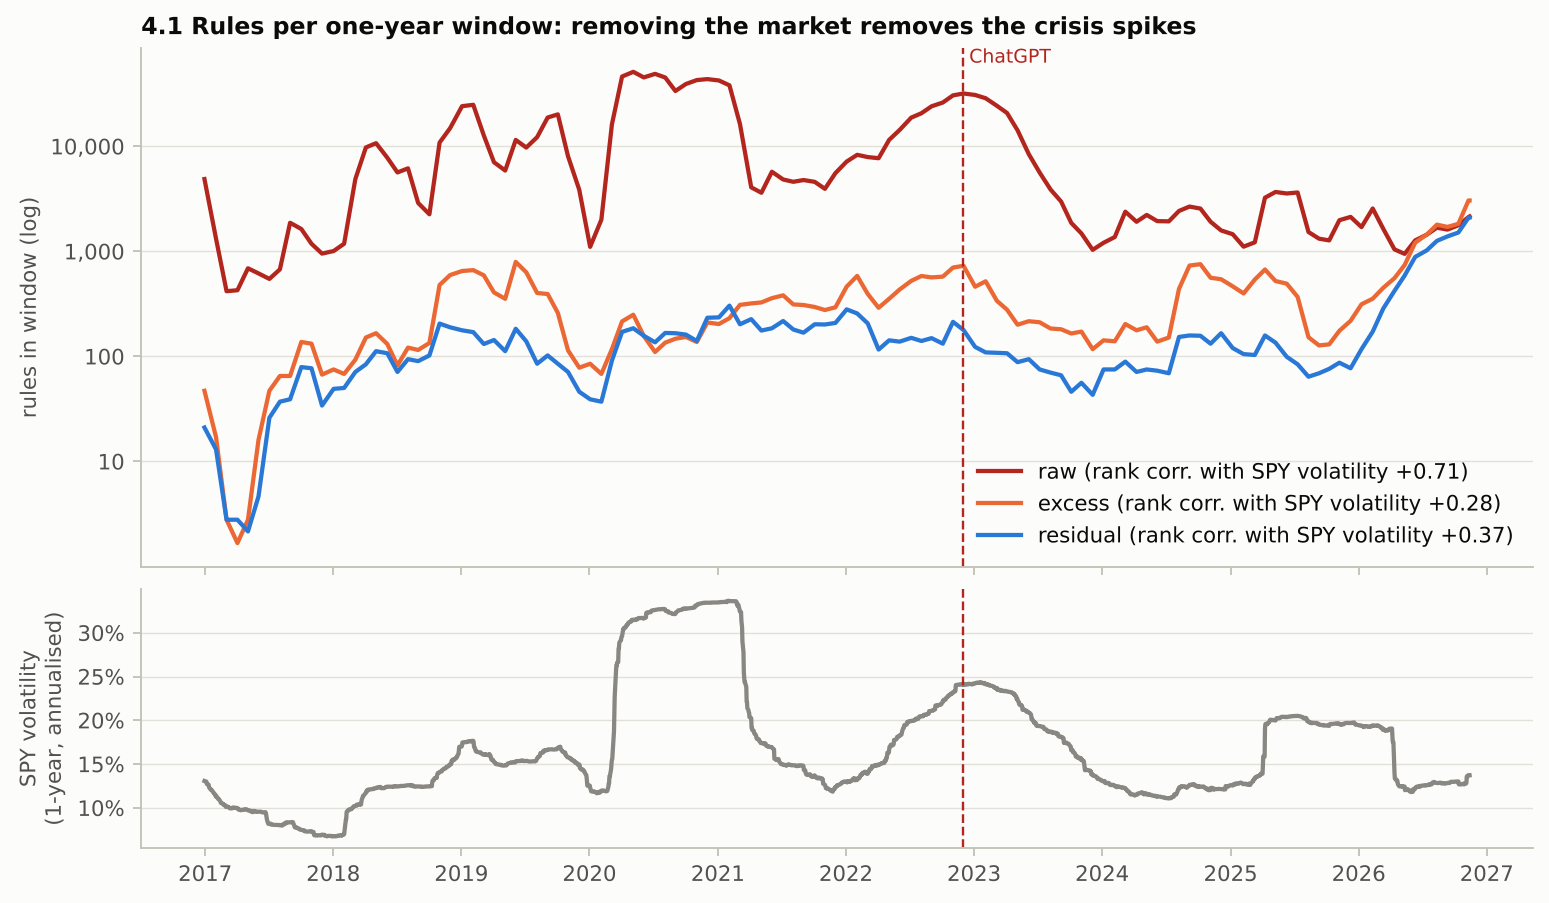
\includegraphics[width=\columnwidth]{4_1_rules_per_window_by_mode.png}
\caption{Rules per one-year window under three return definitions (log scale), with SPY volatility below. Removing the market removes the crisis spikes.}
\label{fig:rules}
\end{figure}

\subsection{Unusual days match events only when we pick the events}
Of the 27 unusual days, 41\% fall on a scheduled release or within a day of a shock, against 14\% for shifted calendars ($p=0.001$; Fig.~\ref{fig:shift}, top). The bar written in advance was 50\%, so H1c is not met, and the match comes almost entirely from the hand-picked shocks (37\% against 2\%). Shocks were listed because the market moved, so this part is close to circular. Scheduled releases alone, the fair test, match 11\% against 13\% by chance ($p=0.70$). The categories describe all 27 days: 10 shocks, 1 jobs-report day, 5 earnings reactions (for example ADSK, $-19.5$ standard deviations on 29 November 2017, and META and MSFT on 31 July 2025), 5 market-stress days in March 2020, 2 earnings days with a quiet reporter and 4 unexplained days (9 June 2017, the most unusual day of the decade, a tech sell-off; 1 December 2016; 4 November 2020, the day after the election; and 2 January 2026). The earnings and stress categories were added after seeing the table and are descriptions, not tests: with 40 companies reporting four times a year, many days are earnings days by chance.

\subsection{Rate decisions move the bank, not the tech groups}
Fed decision days sit at the 62nd anomaly percentile on median and are more unusual than quiet days ($p=0.002$, significant after correction); CPI and jobs days are not ($p=0.80$ and $0.83$). The groups barely react (Fig.~\ref{fig:shift}, bottom): on Fed days the move ratio is 1.18 for AI enablers (interval 1.00--1.37), 1.04 for Big Tech, 1.06 for software and 1.11 for the control group. JPM, the one bank, makes a major move 1.52 times as often as on quiet days (1.14--1.95) and 1.38 times as often on jobs-report days (1.04--1.70), which fits a business whose profits depend on rates~\cite{bernanke2005}. H1b is supported, with a clear limit: one bank among 40 stocks makes rate news almost invisible to the rest. As items, Fed days give two rules, \texttt{FOMC\_DAY}~$\rightarrow$~\texttt{AMD\_UP} (lift 1.92) and \texttt{FOMC\_DAY}~$\rightarrow$~\texttt{AMAT\_UP} (1.78), against 0.05 expected on shifted calendars, but neither survives correction over 9,720 possible right-hand sides.

\subsection{Earnings move the company's own group, but less than an ordinary big move}
After a company's earnings move, peers in its own group follow with mean spillover lift 1.79 (AI enablers), 1.49 (Big Tech), 1.37 (software) and 1.00 (control). After the same companies' big moves on days without earnings the values are higher: 2.41, 1.75, 1.94 and 1.51. Earnings moves are therefore more company-specific than ordinary moves, which is plausible because they carry news about one firm~\cite{foster1981}. H1a is partly supported. Of 573 earnings rules that pass the thresholds, 5 survive correction, and all 5 are stronger than on ordinary days, e.g.\ \{\texttt{EARN\_ASML}, \texttt{ASML\_UP}\}~$\rightarrow$~\texttt{LRCX\_UP} (lift 5.3 against 3.1) and \{\texttt{EARN\_ACN}, \texttt{ACN\_UP}\}~$\rightarrow$~\texttt{CTSH\_UP} (5.4 against 2.8). Two of the five pair companies that often report on the same day (META with MSFT; XOM with AAPL and AMZN), so they may reflect shared report dates rather than spillover.

\subsection{AI launches were ordinary days; AI business news was not}
ChatGPT's release (68th anomaly percentile) and GPT-4's announcement (49th) were ordinary days for these stocks. Nvidia's revenue guidance (99.3rd), the DeepSeek sell-off (99.6th) and Oracle's \$455bn backlog (97.0th) were not, which supports H1d for single days. The same holds for structure: against 107 monthly placebo break dates, ChatGPT ranks above only 21--62\% of them on four measures of structural change (the bar was 90\%), whereas raw returns would have placed it at the 91st percentile, a false break caused by the 2022 bear market. Of the five AI events, only DeepSeek is followed by a lasting change in the whole structure (Section~\ref{sec:h2}).

\subsection{Shocks rarely land on structure breaks}
At the 18 testable shock dates the break score sits at the 55th percentile on average, against 50\% for shifted dates ($p=0.26$; Fig.~\ref{fig:breaks}). Of the eight largest break peaks, only one, the 2016 election, has a listed shock within a month. The largest peak, 9 June 2017, coincides with the most unusual day but with no listed event. The mid- and late-2025 peaks have no listed shock either; the late-2025 one is closest to Caterpillar's earnings reaction (29 October 2025). Single events make days extreme far more often than they change who moves with whom.

\subsection{The few breaks that happen do not heal}\label{sec:h2}
Of the 19 shocks, Brexit has no half-year before it and the three 2025 shocks after DeepSeek are too recent, leaving 15. In the whole structure 12 show no break, 3 a lasting change (the 2016 election, the 2019 yuan devaluation and DeepSeek) and none a temporary one, so H2 is rejected (Fig.~\ref{fig:recovery}). Restricted to pairs that include an AI stock, four sell-offs (February 2018, the March 2018 tariffs and both COVID dates) shook the AI links for less than a year and then recovered, and one change lasted. The counts are fragile: with $z\geq1.5$ they become 2 temporary and 1 lasting, and with raw returns 2 temporary, 0 lasting and 3 partial (Table~\ref{tab:robust}). DeepSeek's verdict rests on only four second-year points, the minimum the rule allows. We read H2 as suggestive: breaks are rare, and we never saw one in the whole structure that healed.

\begin{figure}[t]
\centering
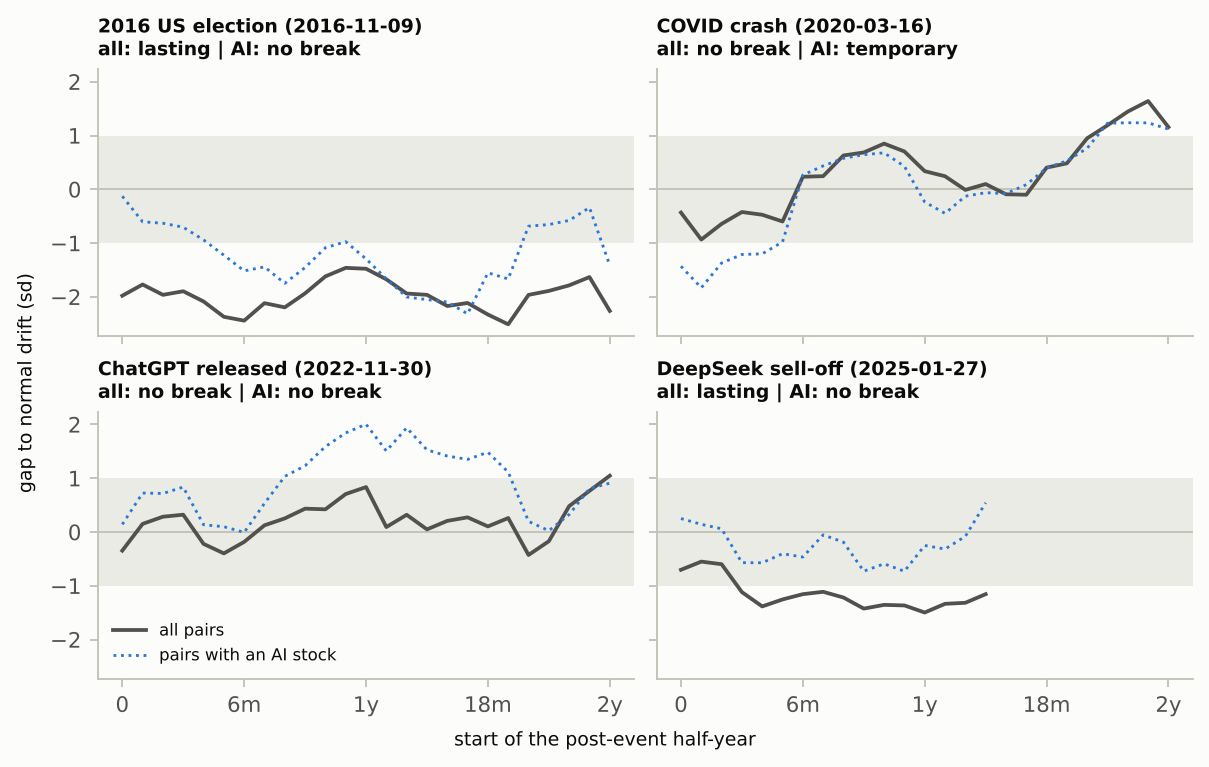
\includegraphics[width=\columnwidth]{7_2_recovery_curves_four_events.png}
\caption{Recovery curves for four shocks: similarity of post-event half-years to the pre-event half-year, as standard deviations from normal drift (band $=\pm1$). Grey: all pairs; blue dotted: pairs with an AI stock.}
\label{fig:recovery}
\end{figure}

\begin{table}[t]
\caption{Event tests under three settings}
\label{tab:robust}
\centering
\footnotesize
\setlength{\tabcolsep}{4pt}
\begin{tabular}{lccc}
\toprule
 & Main & $z{=}1.5$ & Raw \\
\midrule
Days matched (chance 14\%) & 41\% & 41\% & 44\% \\
Shock break pct.\ ($p$) & 55 (0.26) & 64 (0.05) & 51 (0.40) \\
H2 temp./lasting/none & 0/3/12 & 2/1/12 & 2/0/10 \\
\bottomrule
\end{tabular}
\end{table}

\subsection{What did change: the AI category, gradually}
The lasting change we found has no break date. Software--software pair lift rose from 1.47 (year to November 2022) to 2.77 (year to November 2026), while AI--software lift fell from 1.23 to 0.58, below chance. At the stock level (Fig.~\ref{fig:affinity}) two stocks significantly joined the chip-stock cluster, Oracle (affinity 0.59 to 1.65) and Caterpillar (0.98 to 1.80), and 14 left it, mostly software (ADBE, ADSK, NOW, WDAY, INTU) plus QCOM. Neither riser is in our AI group, which is why the groups had to be tested rather than assumed. This is category-based co-movement~\cite{barberis2005}: the market redrew who counts as an AI stock over three years, not on an event day. For a manager, chips, Oracle and Caterpillar are one AI bet, not three diversified ones.

\begin{figure}[t]
\centering
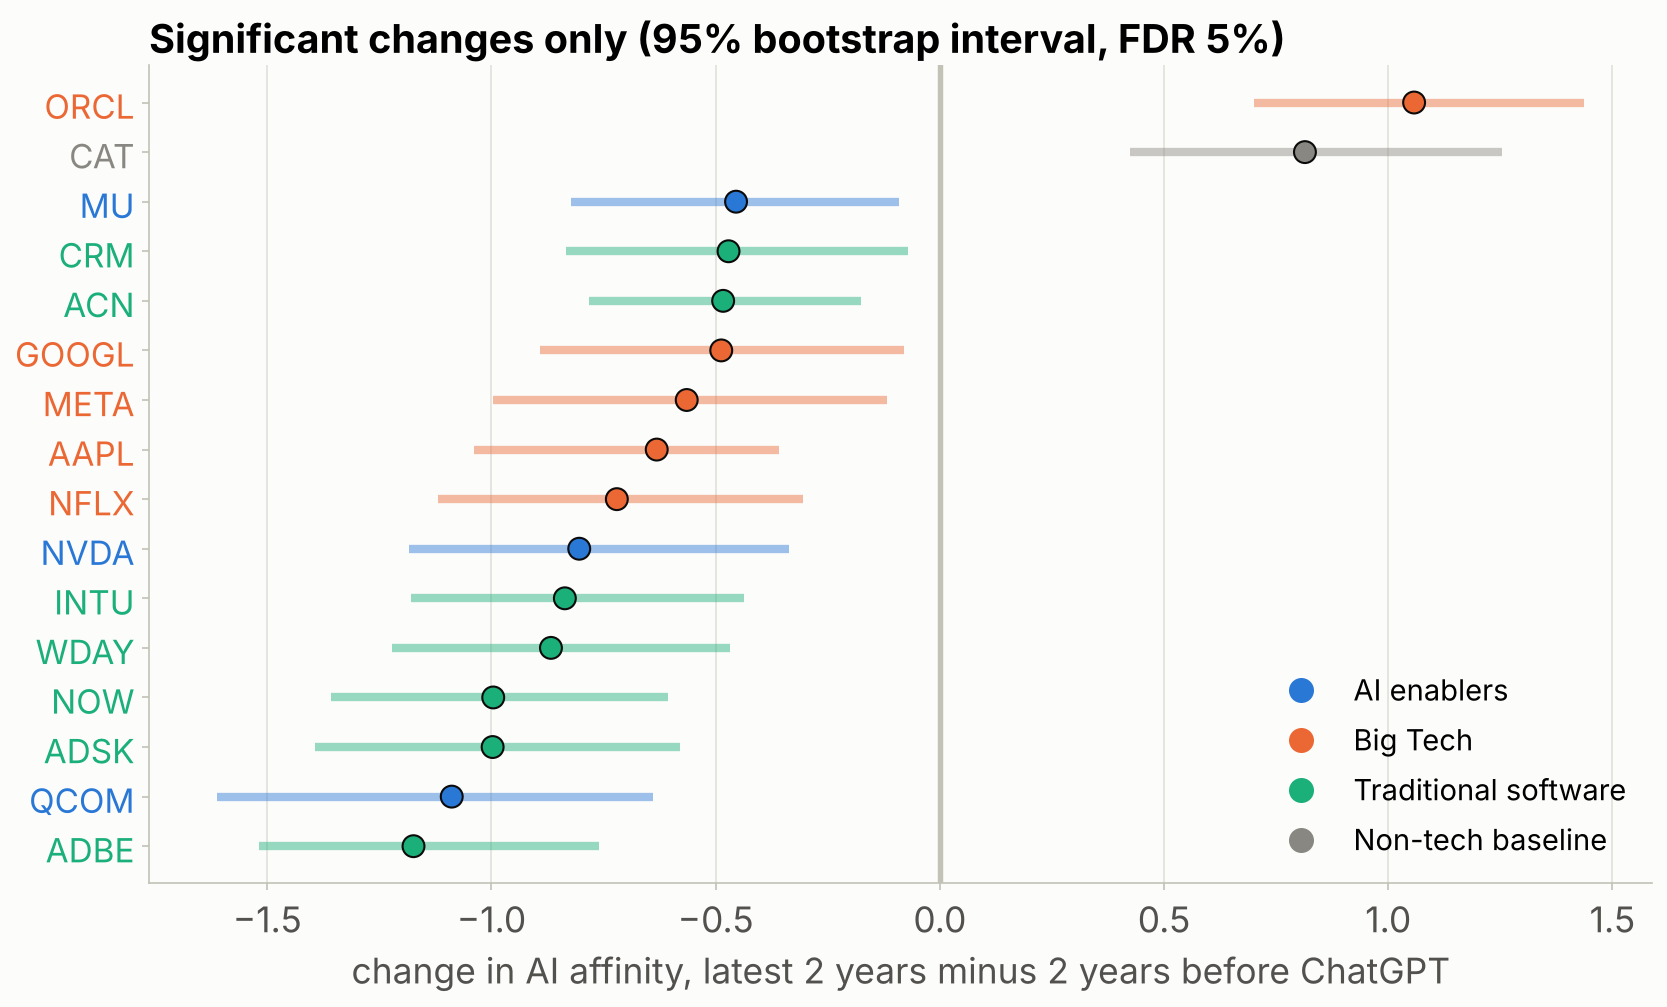
\includegraphics[width=\columnwidth]{affinity.png}
\caption{Stocks whose AI affinity changed significantly between the two years before ChatGPT and the latest two years (95\% block-bootstrap intervals, FDR 5\%). Colours are our groups.}
\label{fig:affinity}
\end{figure}

\subsection{Which rules last}
Of 14,339 labelled rules, 29\% survive the next half-year. Survival rises with age, from 21\% for new rules to 58\% for rules seen in 12 or more earlier windows, and rules inside one group survive 37\% of the time against 10\% for rules that link groups. Trained before ChatGPT and tested after it, the random forest reaches ROC-AUC 0.66 and logistic regression 0.65, while ranking by lift, the usual way to sort rules, gives 0.58 (Table~\ref{tab:models}). Ranking by age alone reaches 0.63, so most of the skill is a rule's history. In a rolling-origin test the models beat lift in every year from 2020 to 2026 (0.63--0.80). This agrees with the event results: durable co-movement is old and local, and shock-born, cross-group links are short-lived. (Predicting next-day price direction from price and rule features failed in a separate notebook, ROC-AUC about 0.50, which is why the target is a rule and not a price.)

\begin{table}[t]
\caption{Rule survival on post-ChatGPT windows (5,215 rules)}
\label{tab:models}
\centering
\small
\begin{tabular}{lccc}
\toprule
Method & ROC-AUC & PR-AUC & Prec@20\% \\
\midrule
Logistic regression & 0.65 & 0.58 & 0.64 \\
Random forest & \textbf{0.66} & 0.59 & 0.63 \\
Gradient boosting & 0.64 & 0.56 & 0.58 \\
\midrule
Rank by age & 0.63 & 0.57 & 0.62 \\
Rank by lift & 0.58 & 0.40 & 0.39 \\
All rules survive & 0.50 & 0.36 & 0.36 \\
\bottomrule
\end{tabular}
\end{table}

\begin{table}[t]
\caption{Hypotheses, written before the event tests, and verdicts}
\label{tab:scorecard}
\centering
\small
\begin{tabular}{p{0.62\columnwidth}l}
\toprule
Hypothesis and finding & Verdict \\
\midrule
H1 Unusual days and breaks fall on events: only hand-picked shocks match days; breaks $p=0.26$ & Partly \\
H1a Earnings move the own group: yes, but less than ordinary moves & Partly \\
H1b Rate news moves rate-sensitive stocks: JPM 1.52$\times$, groups $\approx$1 & Supported \\
H1c $\geq$50\% of unusual days match an event: 41\% & Not met \\
H1d AI launches ordinary, AI business news not: yes for days; only DeepSeek lasting & Partly \\
H2 Most breaks are temporary: 0 of 15 & Rejected \\
\bottomrule
\end{tabular}
\end{table}

\subsection{Questioning the results}
\emph{Chance:} every event result is compared with 1,000 shifted calendars, rules with shuffled baskets, and multiple tests are corrected. Overlapping windows still make neighbouring weeks, placebo dates and survival samples dependent, so those ranks are descriptive, not exact $p$-values. \emph{Hindsight:} the shocks, H1d and the earnings and stress categories were all shaped by knowing what happened; this is why the scheduled releases, which nobody chose, are the result we lead with. \emph{Triviality:} that JPM reacts to the Fed or AMAT moves with LRCX is obvious; the non-obvious findings are that scheduled news does not explain unusual days, that big events rarely change the structure, and that the AI category moved without a break date. \emph{Robustness:} the match rate and the absence of a shock--break link hold in all three settings (Table~\ref{tab:robust}); the H2 counts do not, so we call them suggestive.

\section{Conclusion}
Removing the market before mining is essential: without it, rules track volatility. With it, the strangest days of the decade line up with events only when we pick the events by hand; scheduled Fed, CPI and jobs news is no better than chance, except that Fed days move the one bank. Big events make days extreme but rarely change who moves with whom: 12 of 15 shocks left no mark and none caused a break that healed. The change that did last, the redrawing of the AI category, was gradual. For a manager this means reacting to every news day is not needed; watching slow category shifts and trusting old, within-group rules is.

\textbf{Limitations.} The 40 stocks were chosen by us, all exist today (survivorship bias) and include one bank and one oil company, so rate- and commodity-sensitive reactions are barely measurable. The shock list is a biased sample. Half-year windows cannot see breaks that last only weeks, and shocks after mid-2025 have too little data after them.

\textbf{Future work.} Repeat the event tests on a universe chosen by a fixed rule, the S\&P~100 as it stood in January 2016, which adds banks, utilities and real-estate stocks and removes our own choice of stocks; compare our 40 with random 40-stock draws from it; test H2 rule by rule (do rules born near an event die sooner?); and explain the four unexplained days with news text.

\section*{Code, Data and Acknowledgement}
Code, the price file, the event calendar with its build script and sources, the earnings dates, every figure and table and both key-number files are at~\cite{repo}; \texttt{final\_project.ipynb} and then \texttt{events.ipynb} run top to bottom. Prices and earnings dates were downloaded with \texttt{yfinance}~\cite{yfinance}. Code and text were drafted with the help of an AI assistant (Claude, Anthropic) and reviewed by the authors.

\bibliographystyle{IEEEtran}
\bibliography{refs}

\end{document}
